\documentclass[12pt]{article}
\usepackage{achemso}
\usepackage[margin=1.0in]{geometry}
\usepackage{setspace}
\usepackage{amsmath}             % for equation typesetting
\usepackage{amssymb}             % for equation typesetting
\usepackage{mathrsfs} 
\usepackage{wasysym}             % for geometric shapes
\usepackage{color}               % for colored fonts
\usepackage{setspace}            % for 1.5 and double spacing
\usepackage{graphicx}            % main graphics package
\usepackage{wrapfig}             % allow text wrapping around figures
\usepackage{subcaption}
%\doublespacing
\linespread{1.5}

\usepackage{appendix}

\usepackage[capitalize]{cleveref}
\crefname{figure}{Fig.}{Figs.}
\Crefname{figure}{Figure}{Figures}
\crefname{table}{Tab.}{Tabs.}
\Crefname{table}{Table}{Tables}
\crefname{equation}{Eq.}{Eqs.}
\Crefname{equation}{Equation}{Equations}
\crefname{section}{Sec.}{Secs.}
\Crefname{section}{Section}{Sections}
\crefname{appsec}{appendix}{appendices}
\Crefname{appsec}{Appendix}{Appendixes}

%\usepackage{titlesec}
%\titleformat*{\section}{\Large\bfseries}
%\titleformat*{\subsection}{\large\bfseries}

% Mathematical Shortcuts
\newcommand{\pfrac}[2]{\frac{\partial #1}{\partial #2}}   % partial derivative
\newcommand{\difrac}[2]{\frac{d #1}{d #2}}                % derivative
\newcommand{\bpar}[1]{\left( #1 \right)}                  % big parentheses
\newcommand{\bbra}[1]{\left[ #1 \right]}                  % big brackets
\newcommand{\bbar}[1]{\left| #1 \right|}                  % big bars
\newcommand{\bra}[1]{\left\langle #1 \right\vert}         % bra
\newcommand{\ket}[1]{\left\vert #1 \right\rangle}         % ket
\newcommand{\inner}[2]{\left\langle #1 \left\vert\right. #2 \right\rangle}            % bracket
\newcommand{\innerop}[3]{\left\langle #1 \left\vert #2 \right\vert #3 \right\rangle}  % operator matrix element
\newcommand{\innersub}[4]{\langle \bd{#1}_{#2}, \bd{#3}_{#4} \rangle}                 % bracket with subscripts
\newcommand{\half}{\frac{1}{2}}                           % 1/2
\newcommand{\powfrac}[3]{\bpar{\frac{#1}{#2}}^{#3}}       % fraction raised to a power
\newcommand{\ii}{\infty}                                  % infinity symbol
\newcommand{\tquad}{\quad\quad\quad}                      % triple-quad spacing
\renewcommand{\Im}{\text{Im}}                             % imaginary symbol
\renewcommand{\Re}{\text{Re}}                             % real symbol

\newcommand*\mycommand[1]{\texttt{\emph{#1}}}
\newcommand*\suchthat[0]{\text{ }\vert\text{ }}
\newcommand*\complexmatfield[1]{\mathbb{C}^{#1\text{x}#1}}
\newcommand*\speciallinear[2]{\mathrm{UnL}(#1,#2)}
\newcommand*\complexspeciallinear[1]{\speciallinear{#1}{\mathbb{C}}}
\newcommand*\generallinear[2]{\mathrm{GL}(#1,#2)}
\newcommand*\complexgenerallinear[1]{\generallinear{#1}{\mathbb{C}}}
\newcommand*\mat[1]{\boldsymbol{#1}}

\newcommand*\vc[1]{\boldsymbol{#1}}
\newcommand*\op[1]{\mathcal{#1}}


\title{General Exam}
\date{October 19, 2016 \\ CHB 239}
\author{David Williams-Young\\ Department of Chemistry, University of Washington}


\begin{document}
\linespread{1.0}
\maketitle
\linespread{1.5}


\newpage
\section{Introduction}

Electronic and nuclear motion are fundamental to our understanding of chemical
and physical phenomena. From  geometric reorganization upon photo-induced charge
transfer in the chromophores of photovoltaics  to vibrational mediation of
intersystem crossing that gives rise to phosphorescence,  molecular dynamics
lies at the heart of chemistry.  As such, to properly model these phenomena
theoretically, we must often venture into the time-domain to capture the physics
necessary to completely understand the problem at hand. As such, this task
constitutes a primary focus of modern \emph{ab initio} quantum molecular theory.
{\bf
Although much work has gone into the field of \emph{ab initio} molecular
dynamics, the scope of inquiry has been primarily limited to a non--relativistic
regime.
}

Relativistic effects, while often neglected in most standard treatment of
quantum mechanics, can have profound consequences in chemical
systems.\cite{Pyykko12_45} Scalar relativistic effects cause the contraction of
the core electron shells of heavy atoms, but perhaps of even more consequence is
the introduction of spin couplings in the Hamiltonian.  Spin-spin (SSC) and
spin-orbit (SOC) coupling can affect the electronic spin dynamics even in light
atoms. A direct consequence of these couplings on the electronic manifold is the
breaking of spin--symmetry as the Hamiltonian no longer commutes with the spin
operator, $\op{S}$. This breaking of spin--symmetry is what allows, at an
operator level, for formally spin--forbidden processes to occur, namely
intersystem crossing (ISC) and internal conversion. Although some approaches
have been purposed to account for SOC in the electronic manifold
perturbatively\cite{Thiel14_JCP124101}, these approximation will break down
whenever SOC is non--negligible. Hence a variational approach much be adopted to
account for these interactions in the general case.  Thus to accurately treat
these inherently relativistic and dynamical phenomena theoretically, one must
provide an \emph{ab initio} description of the relativistic effects throughout
the time--evolution of the quantum system.  
{\bf 
In this work, I will outline my proposed research to accurately simulate
\emph{ab initio} relativistic molecular dynamics using correlated wave
functions.
}  

In the quantum mechanical description of molecular systems, neglecting explicit
coupling to a quantized photon field, time evolution of the total molecular wave
function, $\ket{\Psi (t)}$ is governed by the Hamiltonian wave equation 
(in atomic units),
\begin{equation}
\op{H}(t) \ket{\Psi (t)} = i\partial_t \ket{\Psi(t)} \quad,
\label{eq:WaveEq}
\end{equation}
where $\op{H}(t)$ is the time--dependent Hamiltonian, $\partial_t$ is a
partial derivative with respect to time, and $t$ is a time parameter. We have
adopted the standard description of the wave function as a state vector rather
than an explicit function of coordinates. The moieties enclosed in parentheses
are taken to be parameters, i.e. the wave function is parameterized by time.  In
principle, one may solve (in some approximate manner) \cref{eq:WaveEq}
simultaneously for both the electronic and nuclear degrees of freedom
explicitly. This approach is, however, intractable for quantum systems exceeding
more than a few particles. To simplify the solutions of \cref{eq:WaveEq}, one
may formally decompose $\ket{\Psi (t)}$ into a product of nuclear and electronic
wave functions,
\begin{equation} 
\ket{\Psi (t)} = \ket{\Phi(\vc{R}(t),t)}\otimes\ket{\Theta(t)} 
\quad .  
\label{eq:exactSepElecNuc}
\end{equation} 
Here, $\ket{\Phi(\vc{R}(t),t)}$ and $\ket{\Theta (t)}$ are the electronic and
nuclear wave functions respectively and $\vc{R}(t)$ is the expectation value of
the nuclear position operator, $\vc{R}(t) =
\innerop{\Theta(t)}{\hat{\vc{R}}}{\Theta(t)}$.  It should be noted that the
separation of the total molecular wave function in \cref{eq:exactSepElecNuc} is
formally exact\cite{Gross10_PRL123002, Cederbaum08_JCP124101} without loss of
generality in the non-relativistic treatment of quantum mechanics. Even so, the
equations of motion for the time evolution of \cref{eq:exactSepElecNuc} are
wildly complicated\cite{Ghosh15_MP1} and would only be practical for molecules
consisting of a few atoms.  Nevertheless, this explicitly exact treatment allows
one to, at least in in principle, bifurcate the treatment of quantum molecular
dynamics into explicit treatment of the electronic and nuclear time dependence
separately.  Thus, in order to theoretically treat molecular dynamics
accurately, one must be able to treat both the electronic and nuclear degrees of
freedom to some level of accuracy.  This separation will be the underlying
principle of the future directions that I propose in this work.

% Paragraph on the fact that there exsist a shit ton of methods to solve these
% problems but we're going to focus on CAS/MRCI coupled with TSH


I believe that this proposed work is the natural progression from my previous
works in the field the relativistic electronic structure
theory\cite{DBWY16_Accepted1} and non-relativistic non--adiabatic semi-classical
molecular dynamics.\cite{DBWY16_JCTC935,DBWY16_Submitted1} In the following, I
will present a brief overview of the necessary theory for treatment of
non--adiabatic semi-classical dynamics (\cref{sec:TSH}) and the relativistic
Hamiltonian (\cref{sec:X2C}) which will be used throughout this work.
In \cref{sec:pp-X2C,sec:pp-TSH}, I will briefly recall my advances in relevant
fields and how they interconnect to my proposed research.  Finally,
\cref{sec:Future} will outline my plan for the advancement of \emph{ab initio}
non-adiabatic dynamics to correlated relativistic wave functions.

%In the following  I will use indices $i,j,\dots$ to refer to occupied MOs,
%$a,b,\dots$ to refer to virtual MOs, and $p,q,\dots$ to refer to any orbital
%regardless of occupancy.  All MOs are expanded in terms of real atomic-orbitals
%(AO). The Einstein summation convention will be assumed throughout.

\section{Trajectory Surface Hopping}
\label{sec:TSH}

When obtaining the time evolution of the total molecular wave function, it is
often advantageous to work in so called adiabatic basis (the eigenstates of
\cref{eq:WaveEq}) of quantum states,
\begin{equation}
\op{H}(t) \ket{\Psi_I (t)} = E_I(t) \ket{\Psi_I (t)}
\quad \forall t, I \in \mathbb{N},
\label{eq:EigSpec}
\end{equation}
where $\ket{\Psi_I}$ and $E_I$ represent the $I$-th adiabatic wave function and
eigenenergie, respectively. For the purposes of the current discussion, we will
be assuming a discrete eigenspectrum of the Hamiltonian that is smooth over $t$.
Taking the separating of the total wave function in \cref{eq:exactSepElecNuc},
we may rewrite the total wave function as a linear combination of adiabatic
states,
\begin{equation}
\ket{\Psi (t)} = c_I \ket{\Phi_I (\vc{R}(t),t)} \otimes \ket{\Theta_I (t)}
\quad ,
\label{eq:AdiaExp}
\end{equation}
where $\{ c_I \}$ is a set of expansion coefficients, and $\{\ket{\Phi_I}\}$ and
$\{\ket{\Theta_I}\}$ are the sets of electronic and nuclear adiabatic wave
functions, respectively.. Given the entire eigenspectrum of \cref{eq:EigSpec},
the expansion in \cref{eq:AdiaExp} is formally exact, thus the problem now
becomes how to properly obtain the adiabatic electronic and nuclear wave
functions.

There exist a vast plethora of computational methods to treat the nuclear
dynamics to varying degrees of accuracy. In the proposed work, I will restrict
the discussion of these methods to only include those that are semi-classical.
Semi-classical nuclear dynamics algorithms are those that treat the nuclear
motion classically (by some variant of Newton's equations of motion) while
maintaining a quantum description of the electronic degrees of freedom. That is
to say that we may write the nuclear wave function as a product of delta
functions centered at the classical nuclear positions,
\begin{equation}
\inner{\vc{R}}{\Theta_I (t)} = 
  \prod_{A = 0}^{N_\mathrm{atoms}} \delta^3(\vc{R} - \vc{R}_A(t))
  \quad \forall I,
  \label{eq:ClassicalNuclei}
\end{equation}
where $N_\mathrm{atoms}$ is the number of nuclei in the molecule.  This is
often a valid approach, as the nuclei of molecules are orders of magnitude
heavier than the electrons, and thus move much slower. That is not to say that
nuclei are not, strictly speaking, quantized in their time evolution, but
rather that a large proportion of quantum effects in full molecular dynamics
are due to the time dependence of the electrons. Thus it is usually a valid
assumption that the nuclei time evolve classically relative to their electronic
counterparts. That being said, there are cases in which the quantum evolution
of the nuclei must be explicitly treated, such as tunneling in lighter atoms,
in which these semi-classical methods will not suffice to capture the necessary
physics.

Within the semi-classical treatment of molecular dynamics, computational methods
may be further classified as either adiabatic or non-adiabatic. Both of these
classifications may be characterized by their treatment of the transversal of
the manifold of the adiabatic states. Adiabatic time evolution is rooted in
the adiabatic theorem in that, given an initial state that exists as an energy
eigenstate of $\mathscr{H}(0)$, $\ket{\Psi_I(0)}$, at some time $t' > 0$ in the
future, the quantum system will remain in an eigenstate of the
\emph{corresponding} eigenstate of $\mathscr{H}(t')$, $\ket{\Psi_I(t')}$. In
order for this approximation to be valid (although it can be proven that this
assumption is a best an approximation while an exact adiabatic time evolution
cannot exist unless the quantum system does not time-evolve), it is a
necessary and sufficient condition that the individual energy eigenstates do
not couple though the time-derivative operator,
\begin{equation}
\innerop{\Psi_I(t)}{\partial_t}{\Psi_J (t)}
  \stackrel{\mathrm{\mbox{\footnotesize adiabatic}}}{=} 0
  \quad \forall I \not = J,t.
  \label{eq:AdiabaticNAC}
\end{equation}
\Cref{eq:AdiabaticNAC} may be interpreted as an inability to transport
information between energy eigenstates through the so--called non--adiabatic
coupling (NAC) matrix elements within the adiabatic approximation and thus the
inability to leave said eigenstate throughout the time--evolution.  It follows
that non--adiabatic time evolution encompasses those methods which are able to
transport information though the adiabatic manifold through terms such as
\cref{eq:AdiabaticNAC}. By construction, adiabatic time evolution cannot capture
phenomena such as ISC or internal conversion as they are inherently dependent
on the ability to transport information through the adiabatic manifold.  Thus, in
this work, I will only consider a method which is both semi-classical and
non--adiabatic.


Trajectory surface-hopping (TSH) is one of the most widely applied methods for
simulating electronically non-adiabatic dynamics of molecular and
condensed-phase systems.\cite{Barbatti11_1759, Tavernelli14_62, Tully12_22A301,
Tully98_407, Hynes14_97} At its core, TSH is a stochastic algorithm that
controls which electronic state dictates the forces on the nuclei during a
semi-classical molecular dynamics simulation.\cite{Preston71_562} As described in
the seminal works on the method\cite{Tully98_407, Tully90_1061}, via insertion
of \cref{eq:AdiaExp} into \cref{eq:WaveEq}, one may derive an approximate
equation of motion for an electronic superposition state evolving along a
classical nuclear trajectory,
\begin{align}
  &i  \dot{c}_K(t) = H_{KJ}(t) c_J(t) \label{eq:EOMCs} \\
  &H_{KJ}(t) = \delta_{KJ}E_J(\vc{R}(t)) - i d_{KJ}^\xi (t) \dot{R}_{\xi}(t) \label{eq:HamiltonianElec} \\
  &d_{KJ}^\xi = \innerop{\Phi_K(\vc{R}(t),t)}{\nabla^\xi}{\Phi_J(\vc{R}(t),t)} \label{eq:NAC}
  \quad .
\end{align}
Here, $\vc{H}$ is the Hamiltonian expressed in the basis of electronic adiabatic
states. The nuclear position time evolution is governed by Newtonian mechanics,
\begin{equation}
  -\nabla E_c(t) = \vc{m}\ddot{\vc{R}}(t) \label{eq:Newton}
  \quad.
\end{equation}
While $E_J$ in \cref{eq:HamiltonianElec} represents an arbitrary energy
eigenvalue of adiabat $J$, $E_c(t)$ ($c$ indicating ``current") from
\cref{eq:Newton} is the electronic eigenenergy designated by the TSH algorithm
to drive the nuclear evolution at time $t$.  $\vc{m}$ collects the masses for
each nucleus, and $d_{IJ}^\xi$ is the rank-3 NAC tensor that provides an affine
topological connection on the electronic manifold through the nuclear momentum
operator. $\xi$ is an arbitrary nuclear coordinate.

The representation of the separated equations of motion for the electronic and
nuclear degrees of freedom in
\cref{eq:EOMCs,eq:HamiltonianElec,eq:NAC,eq:Newton} are completely general to
any method used to obtain the electronic adiabatic states. There have been many
extensions of this methods to a vast number of different electronic structure
methods. Recently, I have extended this method for use within the
particle--particle Tamm--Dancoff approximation for the description of the
electronic states\cite{DBWY16_Submitted1}, of which results are presented in
\cref{sec:pp-TSH}. Although TSH has been applied to study ISC using perturbative
approaches of accounting for SOC effects, I argue that this treatment is
inherently flawed as the SOC that is argued to be so negligible as to be
treated perturbatively is exactly the term that gives rise to the physical
phenomena that they observe. To properly treat SOC in TSH, one must account for
the SOC in a non--perturbative manner through an \emph{ab initio} treatment of
some relativistic Hamiltonian.

\section{The Exact Two-Component Method}
\label{sec:X2C}

In the relativistic treatment of quantum molecular systems, the Hamiltonian
of interest is that of the Dirac Hamiltonian,
\begin{equation}
\op{H}_D = 
\begin{pmatrix}
  V \otimes \vc{I}_2 && c \text { } p^k \otimes \vc{\sigma}_k \\
  c \text { } p^k \otimes \vc{\sigma}_k && (V - 2mc^2) \otimes \vc{I}_2
\end{pmatrix} \quad ,
\label{eq:DiracHam}
\end{equation}
which describes the relativistic behavior of a single electron (fermion) in the
presence of a scalar potential $V$. Here, $V$ collects all scalar potential
terms, $\vec{p}$ is the momentum operator (acting as an internal vector
potential), $\vec{\vc{\sigma}}$ is a vector whose elements are the Pauli
matrices, and $\vc{I}_2$ is the 2x2 identity matrix. The implicit parametric
dependence on time has been dropped for brevity. The fact that this is a single
particle operator is quite consequential in the relativistic treatment of
molecules in that $\op{H}_D$ describes the mean-field quantum nature of a
single electron in the presence of the $N-1$ other electrons and the nuclei
(encapsulated in $V$). This is due to the fact that, in general, a Lorentz
invariant many--body Dirac equation does not exist if the Coulomb interaction is
taken to be the interaction potential between charges particles. In this work I
will not be explicitly taking into account relativistic retardation effects,
hence this treatment is not completely relativistic. This treatment does,
however, contain the chemically relevant relativistic effects such as
SOC and  scalar relativistic effects.
From the matrix representation of $\op{H}_D$, it is clear to see that it
acts upon a four--dimensional Hilbert space known as a bispinor field ,
$\ket{\Phi^{4c}}$, whose components are themselves two--dimensional,
\begin{equation}
\ket{\Phi^{4c}} = \begin{pmatrix}
 \ket{\Phi_L} \\ \ket{\Phi_S}
\end{pmatrix} \quad.
\end{equation}
Here, $\ket{\Phi_L}$ and $\ket{\Phi_S}$ are the so--called large and small
components of the bispinor respectively, and are both two--dimensional in the
spin manifold (i.e. spinors).

Although it is possible, in principle, to obtain the eigenstates of
\cref{eq:DiracHam} directly, it as often advantageous from a practical as well
as aesthetic perspective to transform the full four component relativistic
equations into a decoupled two component form. This is often convenient as the
resulting expressions closely resemble those found in non--relativistic
electronic structure theory and therefore allow the employment of standard
electronic structure methods with only minor modifications. In general, such a
transformation takes the form of a unitary operator, $\op{U}$, such that
\begin{equation}
\op{U}: 
\op{H}_D \mapsto \begin{pmatrix}
\op{H}_+ && \vc{0}_2 \\ \vc{0}_2 && \op{H}_- 
\end{pmatrix} \quad \text{ and } \quad
\ket{\Phi^{4c}} \mapsto \begin{pmatrix}
 \ket{\Phi^{2c}} \\ \vc{0}_2
\end{pmatrix} \quad.
\end{equation}
Thus making the transformed $\ket{\Phi^{2c}}$ an eigenstate of $\op{H}_+$.
The transformation under $\op{U}$, in effect, folds the contributions from
the small component of the wave function into the large components. In principle,
such a transformation is exact if a proper $U$ may be found. It is the case
that such an exact transformation is not practical to obtain due to the
effective many--body $V$, thus approximate decoupling schemes must be developed.
Several decoupling schemes have been explored in recent years, but in this work
I will only employ the use of the ``exact" two--component (X2C) method, for which
the exact details may be found elsewhere.

Using the X2C transformation method, we are able to obtain a total effecting
two--component Hamiltonian, which may be written in second quantized form,
\begin{equation}
\op{H}_\mathrm{X2C} = h_{pq}^\mathrm{X2C}c_p^\dagger c_q + 
  \frac{1}{2} \inner{pq}{rs} c_p^\dagger c_r^\dagger c_s c_q + V_\mathrm{NN}
  \label{eq:X2CHam}
\end{equation}
where $c_p$ and $c_p^\dagger$ are single spinor particle annihilation and
creation operators respectively. $\vc{h}^\mathrm{X2C}$ is the effective
relativistic core--Hamiltonian which includes both spin--orbit and scalar
relativistic effects, $\inner{\cdot}{\cdot}$, is the Coulomb operator expressed
in the basis of spinor MOs and $V_\mathrm{NN}$ is the nuclear--nuclear repulsion
energy. Expressing \cref{eq:X2CHam} in basis of a single Slater determinant and
expanding each spinor MO in the AO basis ($\lbrace \chi_\mu \rbrace$),
\begin{equation}
\phi_p ( \vc{r} ) = \sum_\mu \chi_\mu(\vc{r}) C_{\mu p}
\qquad
C_{\mu p} = \begin{pmatrix}
C_{\mu p}^\alpha \\ C_{\mu p}^\beta
\end{pmatrix}
\quad , \label{eq:AO2MO}
\end{equation}
we arrive at a relativistic two--component analogue of the Roothaan--Hall
equations familiar to traditional mean--field electronic structure theory,
\begin{align}
&\frac{1}{2}\left(
  F^S_{\mu\nu} \cdot \vc{I}_2 + F^k_{\mu\nu} \cdot \vc{\sigma_k}
\right) C_{\nu p} = (S_{\mu\nu}\cdot \vc{I}_2) C_{\nu p}
\epsilon_p\label{eq:Roothaan}
%\\
%\nonumber \\
%&F^S_{\mu\nu} = \left(
%  2\left( \mu\nu \vert \kappa\lambda \right) - 
%  \left(  \mu\lambda \vert \kappa\nu \right) 
%\right) P^S_{\lambda \kappa} \nonumber \\
%&F^k_{\mu\nu} = -\left(  \mu\lambda \vert \kappa\nu \right) P^k_{\lambda \kappa}\\
%\nonumber \\
%&\vc{P}^S = \frac{1}{2}\mathrm{Tr}_\sigma (\vc{P}\vc{I}_2) \nonumber \\
%&\vc{P}^k = \frac{1}{2}\mathrm{Tr}_\sigma (\vc{P}\vc{\sigma}_k)
%\label{eq:traceRel}\\
%&P_{\mu\nu} = C_{\mu i} C_{\nu i}^\dagger \nonumber
\end{align}
Here, $\vc{S}$ is the AO overlap matrix, 
%and $(\cdot \vert \cdot)$ is the
%Coulomb operator in the AO basis.
and $\{\epsilon_p\}$ is the set of MO
eigenenergies. $\vc{F}^S$,$\vc{F}^k$ and $\vc{P}^S,\vc{P}^k$ are the scalar and
vector parts of the spinor Fock and density matrices in the AO basis
respectively, 
%and are related to the full spinor operators in terms of the spin
%trace, $\mathrm{Tr}_\sigma$, relations of \cref{eq:traceRel}. 
Is important to note that $C_{\mu p} \in \mathbb{C}^2$ (where the $\alpha$ and
$\beta$ indicies represent inseparable spin-up and spin-down components of
$C_{\mu p}$), thus elements of the total spinor density (and thus the spinor
Fock) are 2x2 complex matrices.  \Cref{eq:Roothaan} may be solved
self--consistently to obtain the lowest energy (single) Slater determinantal
description of the many--body system.

The fact that one may write the X2C Hamiltonian in second quantized form makes it
suitable for application to post--self consistent field descriptions of
electronic correlation. Recently, I have extended the particle--particle
Tamm--Dancoff approximation to X2C optimized wave functions to study the fine
structure splittings in atomic and molecular systems, of which results are
presented in \cref{sec:pp-X2C}.


\linespread{1.0}
\section{The Relativistic Particle-Particle Tamm-Dancoff Approximation}
\linespread{1.5}
\label{sec:pp-X2C}
\linespread{1.0}
\section{Trajectory Surface Hopping within the Particle-Particle Tamm-Dancoff Approximation}
\linespread{1.5}
\label{sec:pp-TSH}

While TSH has seen much use since its inception, it is only tractable, if the
electronic structure theory calculations required at each step in the numerical
integration of the molecular equations of motion  can be reasonably afforded.  In an
effort to enable simulation of larger systems, there has been a push recently to
utilize low-scaling, single reference electronic structure methods in TSH
dynamics studies.\cite{Lan15_1360,Rothlisberger07_023001,Li16_935} While TSH
with single reference  methods is well-suited for describing non-radiative
relaxation within the excited state
manifold\cite{Subotnik14_4253,Barbatti14_1395}, most single reference  methods
give a fundamentally flawed description of non-radiative processes that
terminate via internal conversion to the ground electronic state.  Specifically,
methods which represent the ground state by a single Slater determinant and the
excited states as linear combinations of determinants give an incorrect topology
for the ground and excited electronic energy surfaces in regions of the nuclear
configuration space where they approach degeneracy.\cite{Massimo14_3074,
Martinez06_1039} Symmetry-mandated intersections in the ground and excited
states' potential energy surfaces (PES's) can be absent with single reference
methods, so qualitatively incorrect timescales and mechanisms for ground state
recovery processes  can be predicted.  My recent extension of TSH to the pp-TDA
\cite{DBWY16_Submitted1} has shown that a proper treatment of the PES in the
region of a conical intersection leads to qualitatively different results in
the case of excited to ground state inter-conversion over single reference
methods.

\begin{figure}[h!]
  \centering
  \vspace{-0.5cm}
  \begin{subfigure}[b]{0.40\textwidth}
  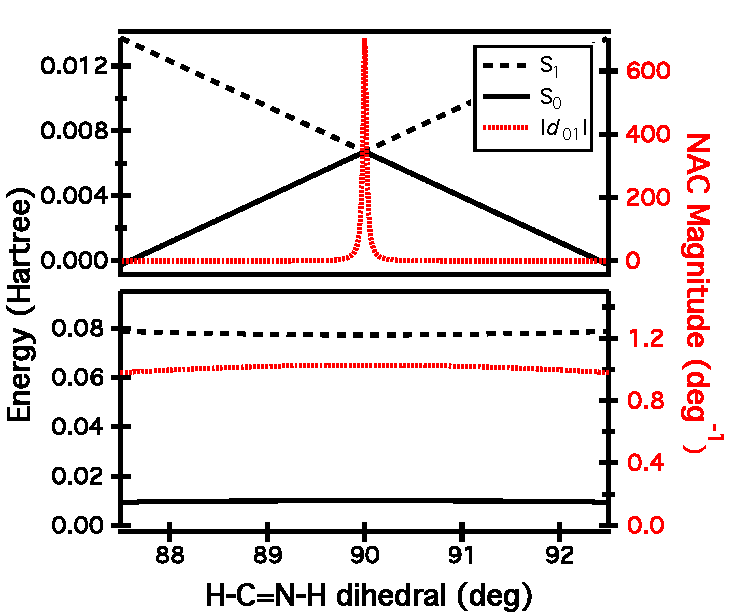
\includegraphics[width=\textwidth]{gs_es_dercp} 
  \caption{ }
  \label{fig:gs_es_dercp}
  \end{subfigure}
  \begin{subfigure}[b]{0.40\textwidth}
  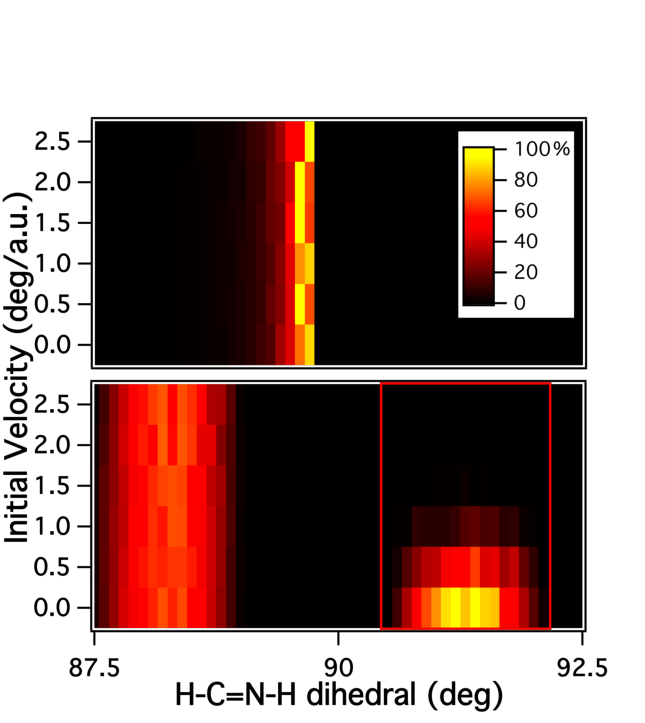
\includegraphics[width=\textwidth]{stacked_hops} 
  \caption{ }
  \label{fig:hops}
  \end{subfigure}
  \caption{\footnotesize (a) Potential energy surfaces for ground and excited
  states, and the coupling strength between the two states with respect to the
  dihedral angle in the vicinity of the minimum energy crossing point between
  S$_0$ and S$_1$ from the pp-TDA (top frame) and CIS (bottom frame) approaches.
  (b) Color maps showing the distribution of configurations at which hops from
  S$_1$ to S$_0$ occur for the different initial velocities resolved at the
  pp-TDA (top frame) and CIS (bottom frame) levels of theory (area in red box
  magnified, after normalization, 1000$\times$ for visibility.)}
\end{figure}

To demonstrate the performance of the pp-TDA within TSH over single reference
methods such as configuration interaction singles (CIS), we simulated the ground
state recovery dynamics for a small iminium ion, H$_2$C=NH$_2^+$, known to
readily photo-isomerize via a conical-intersection-mediated, non-radiative decay
from S$_1$ to the ground state, S$_0$, using both the CIS and pp-TDA description
of the adiabats. The important difference between the two methods is in an
asymmetric treatment of electron correlation in the ground and excited states in
the CIS, while the pp-TDA treats all of the states on the same footing. To
ensure that our dynamics simulation transversed the conical intersection, we
restricted the nuclear trajectories to the well--established isomerization
coordinate of the dihedral rotation.  Potential energy surfaces and coupling
strengths along the reaction coordinate are collected in \cref{fig:gs_es_dercp}. 
There are several conditions for determining the presence of a conical
intersection of PESs. A necessary and sufficient condition is the presence of a
degeneracy as well as a spike in the NAC magnitude in the neighborhood of the
proposed conical intersection (technically the NAC becomes undefined at the
conical intersection which exists at exactly one point on the PES).
It is clear to see that, via these conditions, the conical intersection along
the isomerization coordinate is not captured in the CIS PES, while the pp-TDA
exhibits the correct behavior.

10$^6$ TSH trajectories for a series of 6 initial velocities were considered for
each of the two electronic structure methods.  In all cases the electronic
superposition was initialized as a pure (S$_1$) state, and the dihedral angle
was chosen to be 87.5 degrees so that the dynamics are started in the upper
state near to the region of strongest coupling. Relation profiles for the S$_1$
to S$_0$ inter-conversion are given in the form of a heat plot in
\cref{fig:hops}. There are two characteristics of dynamics in the neighborhood
of conical intersections and are of interest in the relaxation
profiles\cite{Hynes14_97}. First of which is, if the conical intersection is
properly described, internal conversion from S$_1$ $\rightarrow$ S$_0$ should be
localized near the conical intersection. This feature is clearly captured by
the pp-TDA, while CIS suffers a broad relaxation profile that is qualitatively
incorrect. This incorrect profile is due to the artificially early onset of the
NAC along the isomerization coordinate which is a result of improper description
of the conical intersection. The second feature that is important to point out
is that, if the conical intersection is properly described, all of the classical
nuclear trajectories should interconvert before the conical intersection. This
feature is captured in the pp-TDA, even in the initial velocity limit. In the
CIS simulation, a small portion of the trajectories hop at configuration past
the conical intersection at the low initial velocity limit. This means that
those trajectories transversed the conical intersection throughout the
simulation. This qualitatively incorrect behavior would lead to
uncharacteristically long relaxation rates over the pp-TDA.




%Recently, the particle-particle random phase approximation (pp-RPA), a formalism
%for many body correlation energy utilized in the development of modern nuclear
%structure theories\cite{SchuckBook_04}, has been applied to molecular
%systems.\cite{Yang13_030501,Yang13_arXiv1306}  The pp-RPA has also been
%developed to describe the electronic excitation energies using the ground state
%of $N$--2 systems as references.\cite{Yang15_1025} The pp-RPA based methods have
%recently been shown to properly resolve the conical intersection seam between
%the ground and first excited state of H$_3$ along the equilateral
%configurations; a feat not matched by the analogous ph-RPA
%methods.\cite{Yang16_2407} The fact that the pp-RPA methods are able to properly
%predict the proper topology in regions of deneracy, they are well suited for
%application to non--adiabatic dynamics.


%To probe the effects of the mismatched treatment of the ground and excited
%states provided by SR methods on the resulting mixed quantum/classical dynamics,
%we simulated the  ground state recovery dynamics for a small iminium ion,
%H$_2$C=NH$_2^+$, known to readily photo-isomerize via a
%conical-intersection-mediated, non-radiative decay from S$_1$ to the ground
%state, S$_0$, using both a ph-TDA(CIS) and pp-TDA description of the adiabats.
%This is an ideal test case to demonstrate the advantage of the pp-TDA
%description over the analogous ph-TDA.  Since the photoisomerization mechanism
%for this species is well-established, a one-dimensional model potential along
%the isomerization coordinate was chosen to reduce the dimensionality of the
%problem and enforce that the nuclei traverse the conical intersection (or the
%region where the  conical intersection should exist for the ph-TDA).




\linespread{1.0}
\section{Future Directions: Relativistic Electronic Dynamics with Multi-Configurational Wave Functions}
\linespread{1.5}
\label{sec:Future}

\bibliography{Journal_Short_Name,ppSH,Li_Group_References,GE,DBWY,Egidi_References}
\end{document}
